\documentclass[tikz,border=8pt]{standalone}
% Shared look for every TikZ diagram. Load with \input{../../tools/tikz-style.tex}
\usepackage[T1]{fontenc}
\usepackage{lmodern}
\renewcommand{\sfdefault}{lmr}  % diagrams use the same serif as the text
\usetikzlibrary{arrows.meta, positioning, shapes.geometric, calc, fit, backgrounds}
\definecolor{cblue}{HTML}{4C78A8}
\definecolor{corange}{HTML}{F58518}
\definecolor{cgreen}{HTML}{54A24B}
\definecolor{cred}{HTML}{E45756}
\definecolor{cpurple}{HTML}{B279A2}
\definecolor{cgrey}{HTML}{6B6B6B}
\tikzset{
  every picture/.style={font=\sffamily, line width=1.2pt},
  box/.style={draw=#1, fill=#1!12, rounded corners=4pt, align=center, inner sep=7pt, minimum height=1.1cm},
  box/.default=cgrey,
  arrow/.style={-{Stealth[length=3mm]}, draw=cgrey, line width=1.4pt},
  title/.style={font=\sffamily\bfseries\Large},
  note/.style={font=\sffamily\small, text=cgrey, align=center},
}
\AtBeginDocument{\hyphenpenalty=10000 \exhyphenpenalty=10000}

\begin{document}
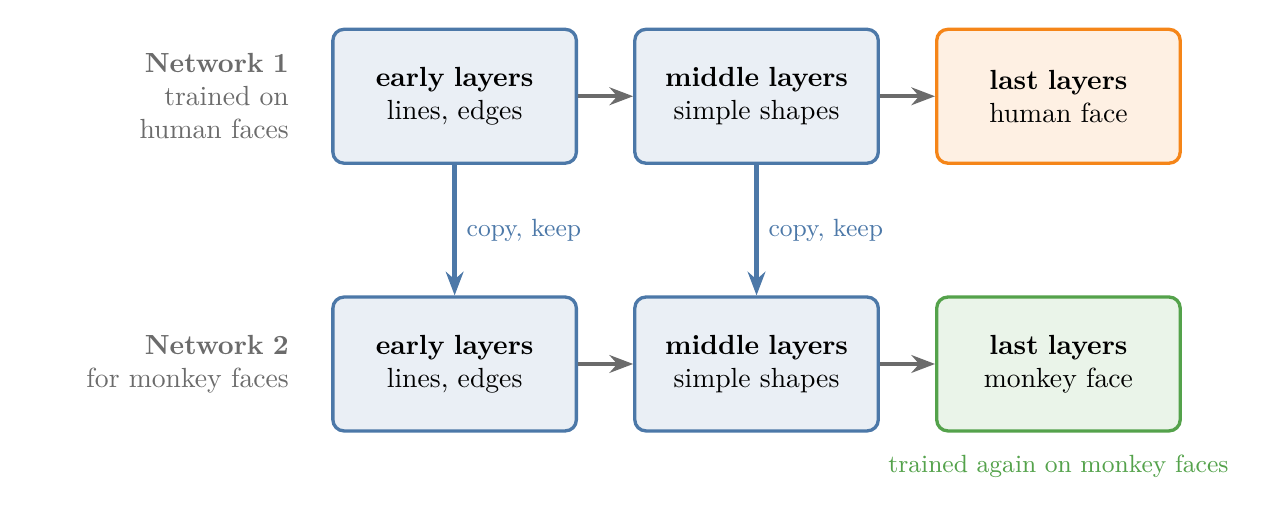
\begin{tikzpicture}[node distance=0.7cm,
  lay/.style={box=#1, text width=2.6cm, minimum height=1.7cm, font=\sffamily\normalsize}]
  % row 1: trained on human faces
  \node[note, anchor=east, font=\sffamily\normalsize, text width=3.2cm, align=right] at (-0.4,0) {\textbf{Network 1}\\trained on human faces};
  \node[lay=cblue, anchor=west] (a1) at (0,0) {\textbf{early layers}\\lines, edges};
  \node[lay=cblue, right=of a1] (a2) {\textbf{middle layers}\\simple shapes};
  \node[lay=corange, right=of a2] (a3) {\textbf{last layers}\\human face};
  \draw[arrow] (a1) -- (a2); \draw[arrow] (a2) -- (a3);
  % row 2: reused for monkey faces
  \node[note, anchor=east, font=\sffamily\normalsize, text width=3.2cm, align=right] at (-0.4,-3.4) {\textbf{Network 2}\\for monkey faces};
  \node[lay=cblue, anchor=west] (b1) at (0,-3.4) {\textbf{early layers}\\lines, edges};
  \node[lay=cblue, right=of b1] (b2) {\textbf{middle layers}\\simple shapes};
  \node[lay=cgreen, right=of b2] (b3) {\textbf{last layers}\\monkey face};
  \draw[arrow] (b1) -- (b2); \draw[arrow] (b2) -- (b3);
  \draw[arrow, cblue, line width=2pt] (a1) -- node[right, font=\sffamily\small, text=cblue] {copy, keep} (b1);
  \draw[arrow, cblue, line width=2pt] (a2) -- node[right, font=\sffamily\small, text=cblue] {copy, keep} (b2);
  \node[font=\sffamily\small, text=cgreen, below=0.15cm of b3] {trained again on monkey faces};
\end{tikzpicture}
\end{document}
